\chapter{DESENHO DO CAMPO DE JOGO E “DIAMOND”}
\label{ap:Campo}

\section{DIMENSÕES OFICIAIS DO CAMPO DE JOGO} 

{\begin{center}
		
\includegraphics[width=.70\textwidth]{fig/campo01}
\end{center}}
\clearpage
\section{DIMENSÕES OFICIAIS DO DESENHO DO “DIAMOND” }

{\begin{center}
		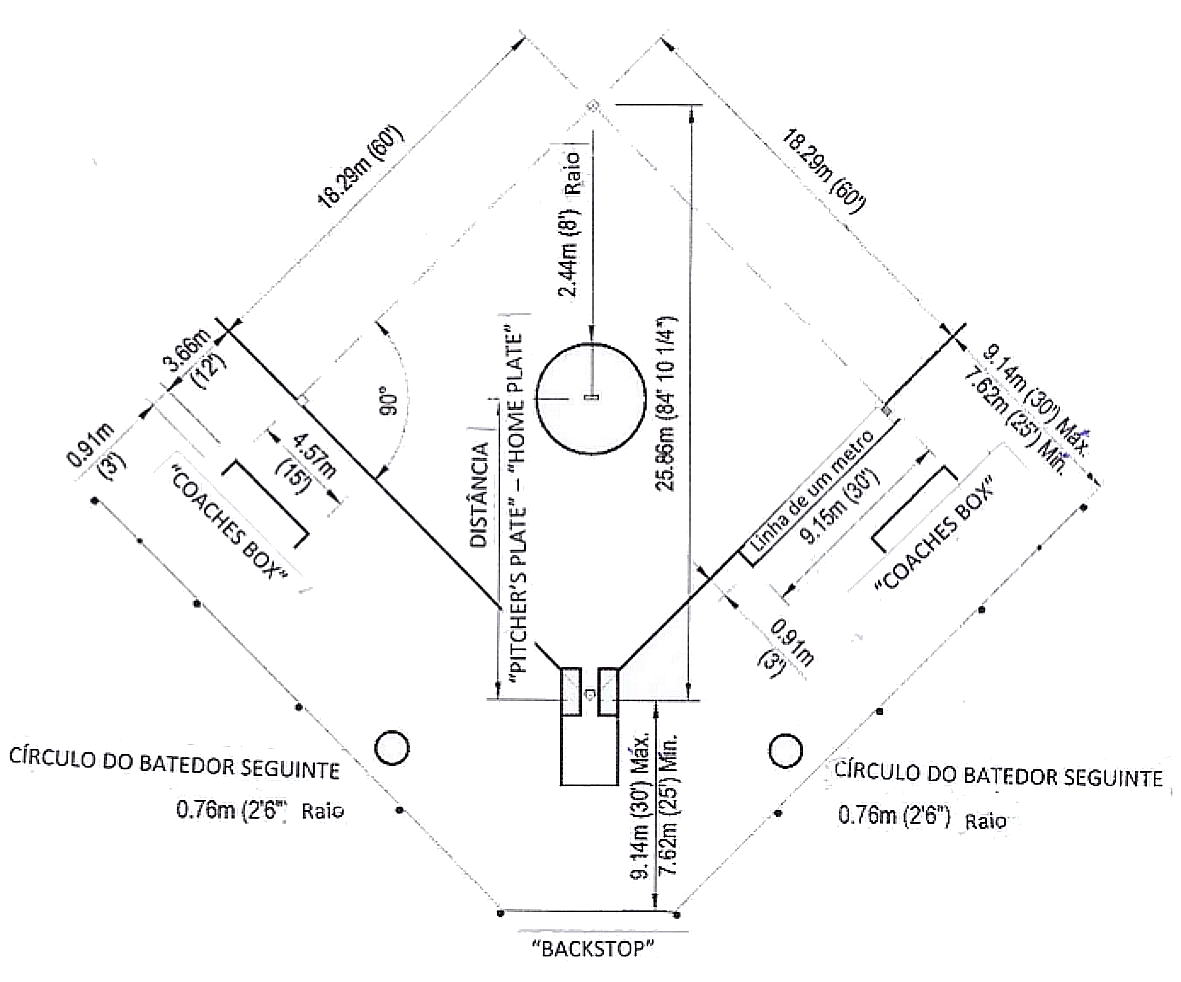
\includegraphics[width=.75\textwidth]{fig/campo02}\end{center}}

\section{DIMENSÕES OFICIAS DAS BASES}
{\begin{center}
		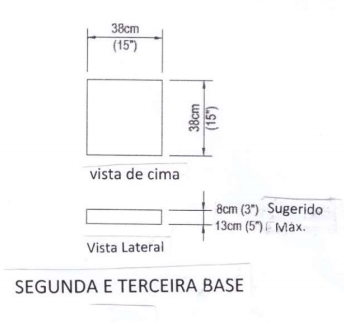
\includegraphics[width=.45\textwidth]{fig/base03}
		
\includegraphics[width=.45\textwidth]{fig/base01}
\end{center}}

\section{DIMENSÕES OFICIAIS DO “BATTER’S BOX” E “CATCHER’S BOX” }
{\begin{center}
		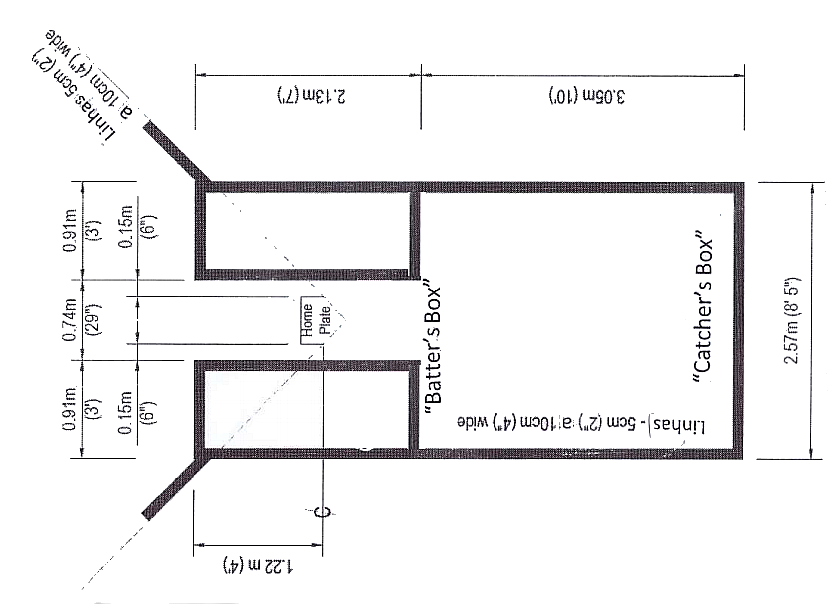
\includegraphics[width=.50\textwidth,angle=180]{fig/catcherbox}\end{center}}

\section[\textit{Home Plate} \Gls{pitcher's plate}]{DIMENSÕES OFICIAIS DO “HOME PLATE” E “PITCHER’S PLATE”}

{\begin{center}
		
\includegraphics[width=.45\textwidth]{fig/home}
		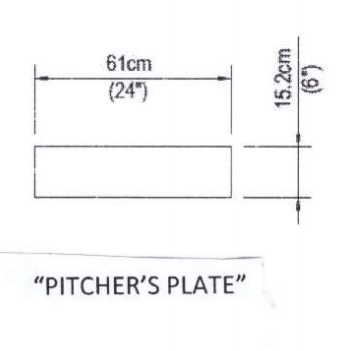
\includegraphics[width=.45\textwidth]{fig/pitcher}
\end{center}}

\section{TABELA DE REFERÊNCIA RÁPIDA}

\resizebox{.95\textwidth}{!}{
	\begin{tabular}{p{40mm}p{160mm}}\footnotesize
		“BACKSTOP” E LINHAS LATERAIS (LINHA DE BOLA MORTA/CERCA LATERAL)& 
		O “backstop” (barreira situada atrás da área do “home plate”) e as linhas/cercas 
		laterais devem estar situadas a 7,62m (25 pés), no mínimo, e a 9,14m (30 pés), no 
		máximo, atrás das linhas de “foul”. A área entre as linhas de “foul” e o “backstop”, e 
		entre as linhas de “foul” e as linhas/ cercas laterais, tem de estar desobstruída. \\\hline
		BASES &
		Distâncias: “Home Plate” até primeira/terceira base: 18,29m (60 pés) da parte de trás 
		da placa até a parte de trás da base. “Home Plate” até segunda base: 25,86m (84 pés 
		10 1/4 polegadas) da parte de trás da placa até o meio da base. As bases devem ser 
		feitas de lona ou outro material apropriado, e devem estar firmemente fixadas em sua 
		posição. 
		
		Metade da Base Dupla (Primeira Base) é fixada em território “fair”, e é parte do 
		território “fair”, e a outra metade (de cor bem diferente e contrastante), em território 
		“foul”, e é parte do território “foul”. \\\hline
		“BATTER’S BOXES” &
		Um em cada parte do “home plate”. Devem medir 0,91m (3 pés) por 2,13m (7 pés). As 
		linhas internas do “batter’s box” devem estar a 15,20cm (6 polegadas) do “home 
		plate”. A linha dianteira do “box” deve estar a 1,22m (4 pés) na frente de uma linha 
		traçada através do centro do “home plate”. As linhas são consideradas dentro do 
		“batter’s box”. \\\hline
		“CATCHER’S BOX” &
		Medida: 3,05m (10 pés) de comprimento dos cantos externos traseiros dos “batter’s 
		boxes” e deve ter 2,57m (8 pés 5 polegadas) de largura. As linhas são consideradas 
		dentro do \gls{catcher's box}.\\\hline 
		“COACHES’ BOXES”& É aquela área atrás de uma linha de 4,57m (15 pés) traçada fora do “Diamond” 
		(campo). A linha é paralela à linha da primeira/terceira base, e está a 3,66m (12 pés) 
		dessas linhas, estendidas das bases em direção ao “home plate”. \\\hline
		TABELA DE DISTÂNCIAS &
		\begin{tabular}{l|c|c|c}
			\multicolumn{2}{c|}{CATEGORIA} &\parbox{30mm}{“H. PLATE”-“P. PLATE”}&\parbox{40mm}{ CERCAS DO CAMPO EXTERNO (mínimas)} \\\hline\hline
			\multirow{2}{*}{J\'unior fem.} 
			&16 anos e $<$ &12,19m (40 pés)&\multirow{3}{*}{ 67,06m (220 pés)} \\\cline{2-3}
			&19 anos e $<$& \multirow{2}{*}{13,11m (43 pés)}& \\\cline{1-2} 
			Feminino 	&			& & \\\hline
			\multirow{2}{*}{J\'unior masc.} 
			&16 anos e $<$&\multirow{3}{*}{14,02m (46 pés)} &\multirow{3}{*}{76,20m (250 pés)} \\\cline{2-2} 
			&19 anos e $<$& &   \\\cline{1-2} 
			Masculino 	&			& &   \\\hline
		\end{tabular}
		\\\hline
		“HOME PLATE” &
		Deve ter cinco lados. A borda voltada para o arremessador deve ter 43,20cm 
		(17polegadas) de largura. Os lados devem ser paralelos às linhas internas do “batter’s 
		box” e devem ter 21,60cm (8 $\frac{1}{2}$ polegadas) de comprimento. Os lados da ponta voltada 
		ao receptor devem ter 30,50cm (12 polegadas) de comprimento. \\\hline
		CAMPO INTERNO &
		“É aquela parte do campo, sem grama, que forma um arco a 18,29m (60 pés)s do 
		centro da borda dianteira do “pitcher’s plate”. LINHAS 
		Devem ter 50mm a 100mm (2 a 4 polegadas) de largura. \\\hline
		CÍRCULO DO BATEDOR PREVENIDO &
		É um círculo com 1,52m (5 pés), 0,76m (2 pés e 6 polegadas) de raio, localizado 
		próximo ao fim da área do “bench” ou “dugout” dos jogadores mais perto do “home 
		plate”. \\\hline
		LINHA DE UM METRO &
		Linha traçada paralelamente à linha de base, e a um metro (3 pés) dessa linha, 
		partindo de um ponto onde inicia a segunda metade da distância entre o “home plate” 
		e a primeira base. \\\hline
		CÍRCULO DO ARREMESSADOR &
		É um círculo de 4,88m (16 pés), com raio de 2,44m (8 pés), traçado do centro da borda 
		dianteira do “pitcher’s plate”. As linhas são consideradas dentro do círculo. \\\hline
		“PITCHER’S PLATE” &
		É feito de borracha e tem 61cm (24 polegadas) de comprimento e 15,2cm (6 
		polegadas) de largura. A parte superior da placa tem de estar no mesmo nível do solo. \\\hline
		ZONA DE ADVERTÊNCIA &
		Deve estar marcada a 3,66m (12 pés), no mínimo, e 4,57m (15 pés), no máximo, da 
		cerca do campo externo e/ou das cercas laterais. A marcação deve ser feita com 
		material (terra, cascalho) equivalente (mas diferente) ao da superfície do campo. O 
		material tem que ser distinguível do material da superfície do campo externo, e deve 
		chamar a atenção dos jogadores quando eles estão se aproximando da cerca. \\\hline
		
	\end{tabular}
}
\section{TRAÇANDO UM “DIAMOND” }

\begin{multicols}{2}
	Esta seção serve como um exemplo para traçar um campo (“diamond”) com distância 
	de 18,29m (60 pés) entre as bases e 14,02m (46 pés) entre o “home plate” e o 
	“pitcher’s plate”. 
	\begin{enumerate}[label= \arabic*)]
		\item  Para determinar a posição do “home plate”, trace uma linha na direção em que 
		deseja situar o campo. Fixe uma estaca no canto do “home plate” mais perto do 
		receptor. Amarre um cordão nessa estaca e dê nós ou marque a corda de outra forma 
		após medir 14,02m (46 pés), 18,29m (60 pés), 25,86m (84 pés e 10 $\frac{1}{4}$ polegadas) e 
		36,58m (120 pés). 
		\item  Coloque o cordão (sem esticar) ao longo da linha diretora e coloque uma estaca 
		onde marca 14,02m (46 pés). Esta será a linha de frente no meio do “pitcher’s plate”. 
		Ao longo da mesma linha, fixe uma estaca onde marca 25,86m (84 pés e 10 $\frac{1}{4}$ 
		polegadas). Este será o centro da segunda base. 
		\item  Coloque o ponto onde marca 36,58m (120 pés) no local determinado para o centro 
		da segunda base e, pegando o cordão no ponto onde marca 18,29m (60 pés), ande 
		para a direita da linha diretora até esticá-lo e pregue uma estaca no ponto onde marca 
		18,29m (60 pés) –este será o canto externo da primeira base, e o cordão, agora, 
		formará a linha entre a primeira e a segunda bases. 
		\item  Segurando, outra vez, o cordão no ponto onde marca 18,29m (60 pés), atravesse o 
		campo e, da mesma maneira, marque o canto externo da terceira base. O “home 
		plate”, a primeira base e a terceira base estão inteiramente na parte interna do campo 
		(“diamond”). 
		\item  Para conferir as medidas do campo (“diamond”), coloque a ponta da corda que 
		marca o “home plate” na estaca da primeira base, e o ponto onde marca 36,58m (120 
		pés), na terceira base. O ponto onde marca 18,29m (60 pés) deve, agora, coincidir com 
		os locais marcados para o “home plate” e a segunda base. 
		\item  Confira todas as distâncias com uma fita métrica metálica sempre que possível. ANEXO 2: 
	\end{enumerate}
\end{multicols}


\chapter{ESPECIFICAÇÕES DO \gls{bat} }

\section{\gls{bat} OFICIAL }\label{sec:bat}
\begin{multicols}{2}
	\begin{enumerate}[label= \arabic*)]
		\item  O \gls{bat} tem de ser feito com uma pe\c{c}a s\'o, com v\'arias pe\c{c}as juntadas 
		definitivamente, ou com duas pe\c{c}as troc\'aveis. 
		\item Quando o \gls{bat} \'e projetado para ser feito com componentes troc\'aveis, tem de levar em conta o seguinte crit\'erio: 
		\begin{enumerate}[label=\roman*.]
			\item os componentes acoplados devem ter um dispositivo de seguran\c{c}a especial para evitar que equipamento com combina\c{c}ões n\~ao aprovadas seja usado no campo; e 
			\item os “bats” confeccionados com combina\c{c}ões de componentes t\^em de seguir os padrões estabelecidos como se fossem um \gls{bat} feito com uma pe\c{c}a s\'o. Os componentes t\^em de seguir os padrões estabelecidos como se fossem partes de um \gls{bat} feito com uma pe\c{c}a s\'o. 
		\end{enumerate}
		\item  Um \gls{bat} pode ser feito com um peda\c{c}o de madeira de lei (madeira dura), ou com um bloco de madeira composto de dois ou mais peda\c{c}os de madeira colados entre si com um adesivo, de tal forma que a dire\c{c}\~ao das fibras de todas as pe\c{c}as seja paralela ao comprimento do "bat". 
		\item  Um “bat pode ser de metal, bambu, pl\'astico, grafite, carbono, magn\'esio, fibra de vidro, cer\^amica, ou qualquer outro material composto aprovado pela WBSC-SD ou ISF Equipment Standards Comission. 
		\item  Um \gls{bat} pode ser laminado, mas deve conter somente madeira ou adesivo, e ter um acabamento perfeito (quando pronto). 
		\item  A parte mais grossa do \gls{bat} (do início da parte cônica at\'e a ponta do \gls{bat}) deve ser redonda e lisa. 
		\item  N\~ao deve ter mais de 86,40cm (34 polegadas) de comprimento, nem pesar mais de 1077,00g (38 on\c{c}as). 
		\item  N\~ao deve ter mais de 5,70cm (2 1/4 polegadas) de di\^ametro em sua parte mais grossa. É permitida uma toler\^ancia de 0,80mm (1/32 polegada) devido \`a dilata\c{c}\~ao que pode haver no material. 
		\item  Um \gls{bat} n\~ao deve ter rebites expostos, pinos, bordas \'asperas ou afiadas, ou qualquer esp\'ecie de prendedor externo que possa apresentar algum risco. Um "bat" de metal n\~ao deve ter rebarbas nem rachaduras. 
		\item  Um \gls{bat} de metal n\~ao deve ter um cabo de madeira. 
		\item  Um \gls{bat} tem de ter uma empunhadura de seguran\c{c}a de corti\c{c}a, fita (fita pl\'astica n\~ao lisa) ou material composto. A empunhadura de seguran\c{c}a n\~ao deve ter menos de 25,40cm (10 polegadas) de comprimento e n\~ao deve se estender mais de 38,10cm (15 polegadas) da extremidade do cabo. É permitido aplicar resina, alcatr\~ao de pinho ou subst\^ancias em spray somente na empunhadura de seguran\c{c}a, para aumentar a sua efici\^encia. A fita aplicada a qualquer "bat" tem de ser em espiral contínua. N\~ao precisa ser uma camada s\'olida de fita. N\~ao deve exceder duas camadas. 
		\item  Se for de metal e n\~ao tiver sido feito em uma s\'o pe\c{c}a, com a extremidade da parte mais grossa fechada, dever\'a ter uma pe\c{c}a de borracha ou pl\'astico vinil, ou outro material aprovado pela WBSC-SD ou ISF Equipment Standards Commission, firmemente colocada nessa parte do "bat". 
		
		\begin{enumerate}[label=\roman*.]
			\item A tampa colocada na extremidade aberta da parte grossa do \gls{bat} tem de estar firme e permanentemente lacrada, para que ela n\~ao possa ser removida por qualquer pessoa, exceto o fabricante, sem danific\'a-la ou destrui-la. 
			\item O \gls{bat} n\~ao deve causar ruídos. Um \gls{bat} que causa ruídos ser\'a considerado um \gls{bat} ilegal. 
			\item O \gls{bat} n\~ao deve ter sinais de adultera\c{c}\~ao. Um \gls{bat} que mostra sinais de adultera\c{c}\~ao ser\'a considerado um \gls{bat} Adulterado. 
		\end{enumerate}
		\item  Um \gls{bat} tem que ter um dispositivo de seguran\c{c}a (sali\^encia arredondada na extremidade do cabo) de, no mínimo, 0,60cm (1/4 de polegada) ressaltando, a um \^angulo de 90 graus, do cabo, e n\~ao deve ter bordas afiadas. O dispositivo de seguran\c{c}a pode ser moldado, torneado, soldado e permanentemente fixo; pode ser coberto com fita. 
		
		\item  Um \gls{bat} que tenha a informa\c{c}\~ao “Bat Oficial Aprovado” ilegível, devido ao desgaste pelo uso, pode ainda ser utilizado se todos os outros aspectos estiverem de acordo com as regras, e desde que isso possa ser constatado com razo\'avel seguran\c{c}a. 
		\item  O peso, a distribui\c{c}\~ao do peso, ou o comprimento do "bat" t\^em de ser estabelecidos permanentemente por ocasi\~ao da fabrica\c{c}\~ao, e n\~ao podem ser modificados de maneira alguma depois disso, excetuando-se algo diferente que esteja especificamente previsto nesta Regra, ou haja uma especifica\c{c}\~ao aprovada pela WBSC-SD ou ISF Equipment Standards Commission. 
	\end{enumerate}
\end{multicols}

\section{\gls{bat} PARA FAZER AQUECIMENTO} 
\begin{multicols}{2}
	É um \gls{bat} (exceto um \gls{bat} oficial) que tem de ser feito com uma pe\c{c}a s\'o, e deve sujeitar-se aos requisitos exigidos aos dispositivos de seguran\c{c}a (empunhadura de seguran\c{c}a e sali\^encia arredondada na extremidade do cabo) do \gls{bat} oficial. Tem de estar marcado "warm-up", com letras de 3,20cm (1 1/4 polegada), na extremidade do 
	cilindro. A extremidade do cilindro tem que ter mais de 5,70cm (2 1/4 polegadas). 
	
\end{multicols}


\chapter{PADRÕES DE BOLA}
\label{ap:Bola}

\section{BOLA OFICIAL}


\begin{multicols}{2} 
	\begin{enumerate}[label= \arabic*)]
		\item  Tem que ser uma bola com formato regular, emendas lisas, pontos de costura não 
		salientes ou com superfície plana. 
		\item Tem que ter um núcleo central feito tanto de fibra longa de paina de primeira 
		qualidade, de uma mistura de cortiça e borracha, de uma mistura de poliuretano, 
		como de outros materiais aprovados pela WBSC-SD Equipment Standards Commission. 
		\item  Pode ser enrolada (manualmente ou a máquina) com fio trançado de boa qualidade 
		e coberta com cola de látex ou borracha. 
		\item Tem que ter uma cobertura costurada com fio encerado de algodão ou linho, colada 
		à bola mediante aplicação de substância aderente na face inferior (da cobertura), ou 
		uma cobertura moldada colada ao núcleo, ou uma cobertura integralmente moldada 
		com o núcleo. As peças moldadas devem ter uma reprodução autêntica da costura 
		aprovada pela WBSC-SD Equipment Standards Commission. 
		\item  Tem que ter uma cobertura da melhor qualidade, feita de couro de cavalo ou vaca 
		curtido em cromo Nº 1, ou de material sintético ou outros materiais aprovados pela 
		WBSC-SD Equipment Standards Commission. 
	\end{enumerate}
\end{multicols}

\section{DIMENSÕES E ESPECIFICAÇÕES}
\begin{multicols}{2} 
	\begin{enumerate}[label= \arabic*)]
		\item  A bola de 30,50cm (12 polegadas), pronta, deve ter entre 30,20cm (11 7/8 
		polegadas) e 30,80cm (12 1/8 polegadas) de circunferência, e deve pesar entre 
		178,00g (6 $\frac{1}{4}$ onças) e 198,40g (7 onças). O tipo “costura plana” deve ter, no mínimo, 
		88 pontos em cada cobertura, costurados pelo método de duas agulhas. 
		\item  A bola pronta deve ter um coeficiente de restituição e um padrão de compressão, 
		que serão determinados e instituídos pela WBSC-SD Equipment Standards 
		Commission. 
		\item  COR significa Coeficiente de Restituição de uma bola quando medido pelo método 
		de teste para medir o Coeficiente de Restituição de bolas da ASTM (American Society 
		for Testing and Materials). 
		\item  A bola de 30,50cm (12 polegadas), com costura branca ou vermelha ou cobertura 
		amarela com um COR de .47 ou menos, deve ser usada em jogos de Campeonato da 
		WBSC-SD, nas seguintes categorias: Adultos (Masculino e Feminino), Júnior (Masculino 
		e Feminino). As bolas devem ter a logomarca da WBSC-SD. 
		\item  Em bolas usadas em Jogos de Campeonato da WBSC-SD, a força de carga exigida 
		para comprimir a bola 0,64cm (0,25 polegadas) não precisa exceder 170,10kg (375 libras) quando tais bolas são testadas de acordo com o método de provas para medir compressão-deslocamento de bolas de softbol da ASTM, método esse aprovado pela WBSC-SD Equipment Standards Commission. 
	\end{enumerate}
\end{multicols}
Abaixo, estão relacionados os padrões estabelecidos para cada bola: 

\resizebox{\textwidth}{!}{\begin{tabular}{*{8}{c}}
		Bola& Cor da bola &Cor da linha &Tam. Mín.& Tam. Max.& Peso mín.& Peso Max. & Marcação \\\hline\hline
		30,50cm& Branca ou& Costura Bca.& 30,20cm& 30,80cm& 178,00g &198,40g&\multirow{2}{*}{LOGO da WBSC-D}\\\cline{1-7}
		(12”)& Tom. Amar &ou Verm.& (11-7/8”)& (12-1/8”)& (6 $\frac{1}{4}$ onças)&(7onças) &
		\\\hline
\end{tabular}}


\chapter{ESPECIFICAÇÕES DA LUVA} \label{chap:Luva}

ESPECIFICAÇÕES DAS DIMENSÕES: 

\begin{center}
	
\includegraphics[width=.5\textwidth]{fig/Luva}
	
	
	\begin{tabular}{c |p{90mm}|r|r}
		&&cm& polegadas \\\hline\hline
		A& Largura da palma parte superior &20,30& 8  \\\hline
		B& Largura da palma parte inferior &21,60& 8 $\frac{1}{2}$ \\\hline 
		C& Abertura da parte superior do trançado &12,70 &5  \\\hline
		D& Abertura da parte inferior do trançado &11,50 &4 $\frac{1}{2}$  e\\\hline
		E& Topo à base do trançado &18,40& 7 $\frac{1}{4}$  \\\hline
		F& Costura da forquilha do primeiro dedo &19,00 &7 $\frac{1}{2}$  \\\hline
		G& Costura da forquilha do polegar &19,00& 7 $\frac{1}{2}$ \\\hline 
		H& Costura da forquilha &44,50& 17 $\frac{1}{2}$  \\\hline
		I& Topo do polegar à borda inferior &23,50 &9 $\frac{1}{4}$  \\\hline
		J& Topo do primeiro dedo à borda inferior &35,60 &14  \\\hline
		K& Topo do segundo dedo à borda inferior &33,70 &13 $\frac{1}{4}$  \\\hline
		L& Topo do terceiro dedo à borda inferior& 31,10& 12 $\frac{1}{4}$  \\\hline
		M& Topo do quarto dedo à borda inferior& 27,90 &11  \\\hline
	\end{tabular}  
\end{center}


\chapter{ÁRBITROS}



\section{INFORMAÇÕES GERAIS PARA ÁRBITROS }
\begin{multicols}{2}  
	\begin{enumerate}[label=\alph*)]
		\item O árbitro não deve ser um membro de nenhuma das equipes. Exemplos: jogador, 
		"coach", técnico, dirigente, anotador ou patrocinador. 
		
		\item  O árbitro deve estar seguro quanto à data, ao horário e ao local do jogo, e deve 
		chegar ao campo de jogo com antecedência de 20 a 30 minutos, iniciar o jogo 
		pontualmente e deixar o campo depois de encerrá-lo. 
		
		\item  O árbitro (masculino e feminino) tem de usar: 
		\begin{enumerate}[label= \arabic*)]
			\item  Uma camisa azul-claro, com mangas longas ou curtas. 
			\item  Meias azul-marinho escuro. 
			\item  Calças azul-marinho escuro. 
			\item  Boné azul-marinho escuro, com a marca WBSC (em letras brancas decoradas com 
			contornos azuis) pregada na frente. 
			\item  Bolsa para bolas azul-marinho escuro (somente árbitro de "home"). 
			\item  Jaqueta e/ou pulôver azul-marinho escuro. 
			\item  Sapatos e cinto pretos. 
			\item  Uma camiseta branca, que deve ser usada por baixo da camisa azul-claro. 
		\end{enumerate}
		
		
		\item  Árbitros não devem usar joias expostas que possam oferecer risco. 
		
		EXCETO braceletes e/ou colares com fins medicinais. 
		
		\item  O árbitro de "home", na modalidade Arremesso Rápido, tem de usar uma máscara para rosto preta, com estofamento preto ou bege, um protetor de garganta preto, um protetor de tórax e caneleiras que protejam também os joelhos. (Pode ser usada uma máscara que já vem dotada de um protetor de garganta na parte inferior da armação.) 
		
		\item  Os árbitros devem apresentar-se aos capitães, técnicos e anotadores. 
		
		\item  Os árbitros devem inspecionar as delimitações do campo de jogo, o equipamento etc. e esclarecer todas as regras de campo para ambas as equipes e seus "coaches". 
		
		\item  Cada árbitro tem o poder de tomar decisões sobre as infrações cometidas a qualquer momento durante o desenrolar da partida, ou enquanto ela está paralisada, até o jogo ser encerrado.
		\item Nenhum árbitro tem autoridade para desprezar ou questionar as decisões tomadas por outro árbitro dentro dos limites de seus respectivos deveres, conforme está especificado nestas regras. 
		
		\item  Um árbitro pode consultar seu companheiro a qualquer momento. Contudo, a decisão final deve ser do árbitro que, mesmo tendo autoridade exclusiva para decidir, recorreu à opinião de outro árbitro. 
		
		\item  Para definir suas respectivas obrigações, o árbitro que julga as bolas arremessadas ("ball" ou "strike") será designado como o "Árbitro de Home", e o árbitro que julga as decisões nas bases, como o "Árbitro de Base". 
		
		\item  O árbitro de "home" e o árbitro de base devem ter a mesma autoridade para: 
		\begin{enumerate}[label= \arabic*)]
			\item Declarar declarado “OUT” um corredor que sai da base antecipadamente. 
			\item Declarar "TIME" para paralisar o jogo. 
			\item Remover, ou expulsar do jogo, um jogador, "coach" ou técnico, por violação de regras. 
			\item Declarar todos os Arremessos Ilegais. 
			\item Determinar e declarar um “Infield Fly”. \textbf{Quando parecer evidente que uma bola batida será um “Infield Fly”, o árbitro deverá declarar, imediatamente, “INFIELD FLY” SE FOR “FAIR”, OBATEDOR É “OUT”, para beneficiar os corredores}.
		\end{enumerate}
		\item  O árbitro deve declarar declarado “OUT” o batedor, batedor-corredor ou corredor, sem esperar por uma apelação para tal decisão, em todos os casos em que esse jogador é declarado “OUT” de acordo com estas regras. 
		
		\item  A menos que haja uma apelação, o árbitro não deve declarar declarado “OUT” um jogador, ou penalizá-lo, por não ter tocado uma base; por ter deixado uma base antecipadamente numa bola \gls{fly} pega no ar; por ter batido fora de ordem; por ter entrado no jogo como substituto sem ser anunciado ao árbitro; por ter reingressado ilegalmente; por ter entrado no jogo como Jogador de Emergência, ou por ter retornado ao jogo após ter sido removido de acordo com a Regra de Jogador de Emergência, sem comunicação ao árbitro; por ter mudado de posições nas bases com outro corredor; ou por ter tentado ir à segunda base depois de chegar à primeira base, conforme está estabelecido nestas regras. 
		
		\item  Os árbitros não devem penalizar uma equipe por infração de uma regra quando a imposição da penalidade pode resultar em vantagem à equipe infratora. 
		
		\item  A inobservância, pelos árbitros, das instruções contidas no Anexo 5 não é motivo para protesto. Estas instruções são normas de procedimento para árbitros. 
	\end{enumerate}
\end{multicols}
\section{SINAIS}
\begin{multicols}{2}  
	\begin{enumerate}[label=\alph*)]
		\item Para indicar que a partida deve começar, ou ser retomada, o árbitro deve declarar "PLAY BALL" e, ao mesmo tempo, sinalizar para o arremessador efetuar o arremesso. 
		
		\item  Para indicar um “STRIKE”, o árbitro deve levantar a mão direita acima do ombro (dobrar o cotovelo, de modo que forme um ângulo de 90 graus) e, ao mesmo tempo, declarar “STRIKE” com voz clara e firme. 
		
		\item  Para indicar um "BALL", não deve ser usado sinal algum com o braço. 
		
		\item  Para indicar a CONTAGEM de "balls" e "strikes", o árbitro deve declarar a quantidade de "balls" primeiro. 
		
		\item  Para indicar um "FOUL", o árbitro deve declarar "FOUL BALL" e estender ambos os braços, verticalmente, acima da cabeça. 
		
		\item  Para indicar uma bola "FAIR", o árbitro deve estender um braço na direção do centro do campo, agitando-o para a frente e para trás, imitando um movimento de bombeamento. 
		
		\item  Para indicar que um batedor ou corredor é “OUT”, o árbitro deve levantar a mão direita, com o punho cerrado, acima do ombro direito. 
		
		\item  Para indicar que um jogador é "SAFE", o árbitro deve estender ambos os braços, horizontalmente, para os lados do corpo, com as palmas das mãos viradas para o solo. 
		
		\item  Para indicar a paralisação da partida, o árbitro deve declarar "TIME" e, ao mesmo tempo, estender ambos os braços acima da cabeça. Os outros árbitros devem confirmar a paralisação da partida, imediatamente, fazendo o mesmo gesto. 
		
		\item  Para indicar uma BOLA MORTA DEMORADA (“DELAYED DEAD BALL”), o árbitro deve estender o braço esquerdo, horizontalmente, mantendo o punho cerrado. 
		
		\item  Para indicar um "TRAPPED BALL", o árbitro deve estender ambos os braços, horizontalmente, para os lados do corpo, com as palmas das mãos viradas para o solo. 
		
		\item  Para indicar que o batedor-corredor (ou corredor) tem direito a duas bases (\gls{ground rule double}), o árbitro deve estender a mão direita acima da cabeça e, ao mesmo tempo, indicar com dois dedos o número de bases concedidas. 
		
		\item  Para indicar um \textit{home run}, o árbitro deve estender a mão direita com o punho cerrado, acima da cabeça, e fazer um movimento circular em sentido horário. 
		
		\item  Para indicar um "INFIELD FLY", o árbitro deve declarar "INFIELD FLY" SE FOR "FAIR", O BATEDOR É “OUT”. O árbitro deve estender um braço acima da cabeça. 
		
		\item Para indicar que o arremessador não deve efetuar o arremesso ("NOT TO PITCH"), o árbitro deve levantar uma mão com a palma da mão virada para o arremessador. Deve ser declarado “NO PITCH” (arremesso nulo) se o arremessador efetua o arremesso enquanto o árbitro está com sua mão na posição mencionada. 
	\end{enumerate}
\end{multicols}

\chapter{ANOTAÇÃO }

\section{\textit{BOX SCORE}}

\footnote{N.T.: REGISTRO DE DADOS }
\begin{multicols}{2} 
	
	\begin{enumerate}[label=\alph*)]
		\item O nome de cada jogador e a posição, ou posições, a ser(em) ocupada(s) devem ser relacionadas na ordem em que ele bateu, ou teria batido, a menos que o jogador seja substituído legalmente, expulso ou removido do jogo, ou o jogo termine antes de sua vez de bater.
		
		Quaisquer dados estatísticos acumulados pelo Jogador de Emergência enquanto estava no jogo são creditados a esse jogador, mesmo que ele seja um substituto constante da lista que, eventualmente, não entre no jogo para substituir outro jogador. 
	\end{enumerate}
	\textbf{Quaisquer dados estatísticos acumulados por um Corredor Temporário devem ser creditados ao jogador por quem ele está correndo.} 
	\begin{enumerate}[label= \arabic*)]
		\item  O Jogador Designado (JD) é opcional, mas, se vai utilizar um, seu nome tem de ser anunciado antes do início do jogo e estar relacionado no Formulário de Anotações, na ordem correta em que vai atuar como batedor. Serão relacionados dez nomes, e o décimo nome será o do “JOGADOR FLEX” por quem o JD está batendo. 
		\begin{enumerate}[label=(\alph*)]
			\item Os dados referentes à atuação de cada jogador, na ofensiva e na defensiva, têm de 
			estar tabulados. 
		\end{enumerate}
		\item A primeira coluna deve indicar o número de vezes que cada jogador atua como batedor ("at bat"), mas não deve ser imputado um "at bat" contra o jogador quando esse batedor 
		\begin{enumerate}[label= (\alph*)]
			\item Bate um \gls{fly de sacrificio} que ocasiona a marcação de um ponto. 
			\item É autorizado a ‘andar’ (“walk”, “base on balls”). 
			\item É autorizado a ir à primeira base por ter sofrido Obstrução. 
			\item Executa um "bunt" de sacrifício. 
			\item É atingido por uma bola arremessada (\textit{hit by pitch}). 
		\end{enumerate}
		\item A segunda coluna deve indicar a quantidade de pontos anotados por cada jogador. 
		\item A terceira coluna deve indicar a quantidade de \textit{base hits}\footnote{N.T.: batidas indefensáveis}
		batidos por cada jogador. Uma batida indefensável é aquela que permite que o 
		batedor chegue a salvo ("safe") a uma base. 
		\begin{enumerate}[label= (\alph*)]
			\item Quando um batedor-corredor chega a salvo ("safe") à primeira base, ou a qualquer base subsequente, numa bola "fair" que fica no campo, transpõe a cerca, ou atinge a cerca antes de ser tocada por um defensor. 
			\item Quando um batedor-corredor chega a salvo ("safe") à primeira base numa bola “fair” –muito forte, ou muito lenta, ou que dá um salto incomum– impossível de ser defendida por um defensor, com um esforço normal, a tempo de eliminar esse batedor-corredor. 
			\item Quando uma bola "fair" que não tenha tido contato com um defensor se torna "morta" por ter tocado o corpo ou a roupa de um corredor ou árbitro. 
			\item Quando o defensor tenta, sem sucesso, eliminar um corredor precedente e, na opinião do anotador, o batedor-corredor não teria sido declarado “OUT” na primeira base com uma defesa perfeita. 
			\item  Quando o batedor termina o jogo com uma batida indefensável que empurra os pontos necessários para colocar a sua equipe em vantagem no placar, a ele deve ser creditado somente um "base hit" de tantas bases quantas tiver avançado o corredor que anotou o ponto da vitória, com a condição de que ele (o batedor) avance o mesmo número de bases. 
		\end{enumerate}
		
		EXCEÇÃO: Quando o batedor termina o jogo com um \textit{home run} batido para fora do campo, ele deve ser creditado com um \textit{home run}, e todos os corredores, incluindo ele, devem ser autorizados a anotar ponto. 
		
		\item A quarta coluna deve indicar a quantidade de adversários declarado “OUT”s por 
		cada jogador ("put out"). 
		\begin{enumerate}[label= (\alph*)]
			\item Um "put out" é creditado a um defensor cada vez que ele: 
			\begin{enumerate}[label= (\arabic*)]
				\item Pega uma bola batida para o ar (\gls{fly}) ou uma batida em linha reta ("line drive"). 
				\item Pega uma bola lançada que elimina um batedor ou corredor. 
				\item Toca um corredor com a bola quando esse corredor está fora da base na qual tem o direito de permanecer. 
				\item Está mais perto da bola quando um corredor é declarado “OUT” por ter sido 
				atingido por uma bola "fair" ou por ter estorvado um defensor. 
				\item Está mais perto do jogador substituto não anunciado, que é declarado “OUT” de 
				acordo com a Regra 3.2.8. 
				\item Está mais perto de um corredor que é declarado “OUT” por correr fora do caminho da base. 
			\end{enumerate}		
			\item Um "put out" é creditado ao receptor 
			\begin{enumerate}[label= (\arabic*)]
				\item Quando é declarado um terceiro "strike". 
				\item Quando o batedor não bate na ordem correta. 
				\item Quando o batedor interfere na ação do receptor. 
				\item Quando o batedor é declarado “OUT” por ter batido ilegalmente. 
				\item  Quando o batedor é declarado “OUT” em razão de uma tentativa de “bunt” depois de dois “strikes” ter resultado em “foul ball”. 
				\item Quando o batedor é declarado “OUT” por usar um "bat" ilegal ou Adulterado. 
				\item Quando o batedor é declarado “OUT” por ter mudado de um "batter's box" a outro. 
			\end{enumerate}	
		\end{enumerate}
		\item A quinta coluna deve indicar a quantidade de assistências (“assists”) dadas nas 
		eliminações por cada defensor. Deve ser creditada uma assistência 
		\begin{enumerate}[label= (\alph*)]
			\item A cada jogador que maneja a bola em qualquer série de jogadas que resulte na 		eliminação do corredor. Deve ser atribuída somente uma assistência –não mais–a um 		jogador que maneja a bola em qualquer eliminação. Um jogador que tenha auxiliado 		numa Jogada de Perseguição ("Run-Down Play") ou outra jogada do gênero pode ser 		creditado com um “assist” e um "put out". 
			\item A cada jogador que maneja, ou lança, a bola de tal maneira que poderia ter 		contribuído na eliminação de um corredor se não ocorresse um erro subsequente de 		um companheiro de equipe. 			
			\item A cada jogador que, desviando uma bola batida, ajuda na eliminação de um 
			corredor. 
			\item A cada jogador que maneja a bola numa jogada que resulte na eliminação de um 
			corredor, por Interferência, ou por correr fora da linha de base. 
		\end{enumerate}
		
		\item A sexta coluna deve indicar a quantidade de erros cometidos por cada jogador. Erros 
		são registrados nas seguintes situações: 
		\begin{enumerate}[label= (\alph*)]
			\item A cada jogador que executa uma má jogada ("misplay") que prolongue o turno do 
			batedor, ou a vida de um corredor que está ocupando alguma base. 
			\item Ao defensor que deixa de tocar a base após receber a bola para eliminar o 
			corredor, numa Jogada Forçada ou quando esse corredor é obrigado a retornar à base. 
			\item Ao receptor, se um batedor é autorizado a ir à primeira base por Obstrução. 
			\item Ao defensor que deixa de completar uma Jogada Dupla ("Double Play") por ter 
			derrubado a bola. 
			\item Ao defensor, se um corredor avança uma base em razão da falha desse defensor 
			em parar ou tentar parar uma bola lançada corretamente a uma base, contanto que tenha havido motivo para o lançamento. Quando mais de um jogador poderia ter 
			recebido o lançamento, o anotador tem de determinar a quem atribuir o erro. 
		\end{enumerate}
	\end{enumerate}
\end{multicols}

\section[Bat Indefens\'aveis]{NÃO DEVEM SER REGISTRADOS \textit{base hits} (BATIDAS INDEFENSÁVEIS) }
\begin{multicols}{2} 
	Não deve ser anotado um "base hit" nos seguintes casos: 
	
	\begin{enumerate}[label=\alph*)]
		\item Quando um corredor é declarado “OUT” em Jogada Forçada, ou teria sido declarado 
		“OUT” em Jogada Forçada se um defensor não tivesse cometido erro. 
		
		\item  Quando um jogador que pega uma bola batida elimina um corredor precedente com 
		um esforço normal. 
		
		\item  Quando um defensor tenta, mas não consegue eliminar um corredor precedente e, 
		na opinião do anotador, o batedor-corredor poderia ter sido declarado “OUT” na 
		primeira base. 
		
		\item  Quando um batedor-corredor chega a salvo ("safe") à primeira base porque um 
		corredor precedente é declarado “OUT” por ter interferido numa bola batida ou na 
		ação de um jogador da defensiva. 
	\end{enumerate}
	EXCEÇÃO: Se, na opinião do anotador, o batedor teria chegado a salvo ("safe") à 
	primeira base se não tivesse ocorrido a Interferência, a ele deve ser creditado um "safe 
	hit" (batida por meio da qual o batedor-corredor chega a salvo à primeira base). 
\end{multicols}

\section{FLY DE SACRIFÍCIO }
\begin{multicols}{2}
	É anotado um \gls{fly de sacrificio} quando, com menos de dois “outs”, 
	
	\begin{enumerate}[label=\alph*)]
		\item O batedor empurra um ponto com um “fly” que é pego no ar; ou 
		
		\item  Um corredor anota ponto depois que um defensor do campo externo (ou um 
		defensor do campo interno que tenha corrido para o campo externo) derruba um \gls{fly} 
		ou "line drive" após ter tocado a bola, e, na opinião do anotador, esse corredor 
		poderia ter pisado o “home plate”, mesmo que o defensor a tivesse pego no ar. 
	\end{enumerate}
\end{multicols}
\section{PONTOS EMPURRADOS (\textit{run batted in}) }
\begin{multicols}{2} 
	São os pontos anotados por meio de: 
	
	\begin{enumerate}[label=\alph*)]
		\item Um \textit{safe hit}. 
		
		\item  Um "bunt" de sacrifício ou um \textit{slap hit} (SOMENTE AR), ou um \gls{fly de sacrificio} (AR e AL). 
		
		\item  Um \textit{foul fly} pego no ar.
		\item Um "infield put out" (eliminação feita no campo interno) ou "fielder's choice" 
		(opção feita por um defensor na hora de executar uma jogada). 
		
		\item  Ocorrências que forçam um corredor a avançar para "home": por causa de 
		Obstrução, porque o batedor é atingido por uma bola arremessada (\textit{hit by pitch}), ou 
		em razão da concessão de uma base por “balls”. 
		
		\item  Um \textit{home run} e todos os pontos anotados como decorrência desse \textit{home run}. 
	\end{enumerate}
\end{multicols}
\section{ARREMESSADOR CREDITADO COM UMA VITÓRIA }
\begin{multicols}{2} 
	Um arremessador será creditado com uma vitória, nas seguintes situações: 
	
	\begin{enumerate}[label=\alph*)]
		\item Quando, na condição de arremessador abridor, tiver arremessado pelo menos 
		quatro “innings”, e sua equipe, que estava ganhando no momento em que foi 
		substituído, permanecer liderando o placar pelo resto do jogo. 
		
		\item  Quando, numa partida encerrada depois de jogados cinco “innings”, o arremessador 
		abridor tiver arremessado pelo menos três “innings”, e sua equipe tiver anotado mais 
		pontos do que a outra no momento em que a partida é dada por terminada. 
	\end{enumerate}
\end{multicols}
\section{ARREMESSADOR DEBITADO COM UMA DERROTA }
\begin{multicols}{2} 
	Um arremessador será debitado com uma derrota, independentemente do número de 
	“innings” que tenha arremessado, se for substituído quando sua equipe está perdendo 
	e, depois disso, ela não consegue empatar ou tomar a dianteira no placar. 
\end{multicols}
\section{RESUMO DO JOGO }
\begin{multicols}{2} 
	O resumo deve relacionar os seguintes itens, nesta ordem: 
	
	\begin{enumerate}[label=\alph*)]
		\item A quantidade de pontos por "inning" e a contagem final. 
		
		\item  Os pontos empurrados (\textit{run batted in}) e quem os empurrou. 
		
		\item  “Hits" de duas bases ("two-base hits") e quem os bateu. 
		
		\item  "Hits" de três bases ("three-base hits") e quem os bateu. 
		
		\item  "Home runs" e quem os bateu. 
		
		\item  \Gls{fly de sacrificio} (\textit{sacrifice flies}) e quem os bateu. 
		
		\item  Jogadas Duplas ("Double Plays") e os jogadores que delas participaram. 
		
		\item  Jogadas Triplas ("Triple Plays") e os jogadores que delas participaram. 
		
		\item  Quantidade de "walks" (“base on balls”) concedidos por cada arremessador.
		\item Quantidade de batedores declarado “OUT”s por "strike" ("strikeouts") por cada 
		arremessador. 
		
		\item  Quantidade de "hits" e pontos permitidos por cada arremessador. 
		
		\item  O nome do arremessador vencedor. 
		
		\item  O nome do arremessador perdedor. 
		
		\item  O tempo de duração do jogo. 
		
		\item  Os nomes dos árbitros e anotadores. 
		
		\item  Bases roubadas ("stolen bases") e por quem. 
		
		\item  “Bunts" de sacrifício. 
		
		\item  Os nomes dos batedores atingidos por uma bola arremessada e dos arremessadores 
		que os atingiram. 
		
		\item  A quantidade de “wild pitches” feitos por cada arremessador. 
		
		\item  A quantidade de "passed balls" feitos por cada receptor. 
	\end{enumerate}
\end{multicols}
\section{BASES ROUBADAS} 
\begin{multicols}{2} 
	(SOMENTE AR) Deve-se creditar uma base roubada ("stolen base") a um corredor, 
	sempre que ele avança uma base sem a ajuda de um "hit", um "put out", um erro, uma 
	eliminação forçada, um "fielder's choice", um "passed ball", um "wild pitch" ou um 
	arremesso ilegal. Isso inclui um batedor-corredor que avança à segunda base numa 
	base por “balls” concedida. 
\end{multicols}

\section{DADOS DE JOGOS CONFISCADOS ("FORFEITED GAMES")} 
\begin{multicols}{2} 
	Todos os dados de um jogo confiscado devem ser incluídos nas anotações oficiais, 
	exceto aquele registro de arremessador ganhador/perdedor. 
\end{multicols}


\chapter{NOMENCLATURA DAS ATLETAS NAS POSIÇÕES DO CAMPO}

\begin{figure}[!ht]
	\caption{Posicionamento das atletas}
	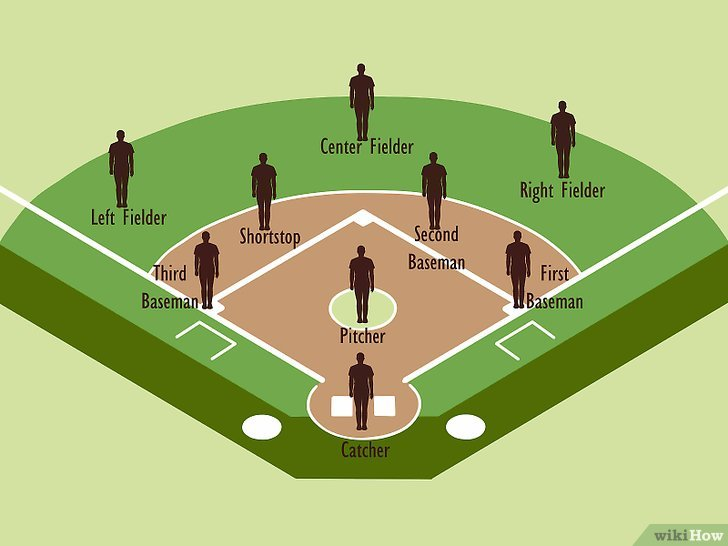
\includegraphics[width=.8\textwidth]{fig/v4-728px-Play-Softball-Step-4-Version-3}
	
	\par Fonte:\url{https://pt.wikihow.com/Jogar-Softbol}
\end{figure}


\chapter{JAPONGLÊS}



\begin{table}[!ht]
	\begin{center}
		\begin{tabular}{lll}
			Japonglês & Inglês      & Português               \\\hline\hline
			Bora      & Ball        & Bola                    \\\hline
			Globo     & Glove       & Luva                    \\\hline
			Polo      & Pole        & Poste                   \\\hline
			Quiátia   & Catcher     & Receptor                \\\hline
			Fasto     & First       & Primeira base           \\\hline
			Secando   & Second      & Segunda base            \\\hline
			Sado      & Third       & Terceira base           \\\hline
			Shoto     & Shortstop   & Interbase               \\\hline
			Gaiá      & Outfielder  & Jardineiro              \\\hline
			Naiá      & Infielder   & Jogador da linha        \\\hline
			Homoran   & Home run    & Rebatida quádrupla      \\\hline
			Guetso    & Get two     & Eliminação dupla        \\\hline
			Tsuberi   & Dive        & Mergulho                \\\hline
			Cabo      & Curveball   & Bola curva              \\\hline
			Naco      & Knuckleball & Arremesso com as juntas \\\hline
			Chenjapo  & Change-up   & Bola lenta              \\\hline
			Furai     & Fly         & Bola alta               \\\hline
			Goro      & Ground      & Bola para o chão       \\\hline
			Yakyuu    & Baseball	& Basebol
		\end{tabular}
		
		\vspace{5mm}
		\footnotesize{Fonte: https://esporte.uol.com.br/olimpiadas/ultimas/2004/07/21/ult2250u4.jhtm}
	\end{center}
\end{table}

\newpage

\begin{table}[!ht]
	\begin{center}
		
		
		\begin{tabular}{lll}
			\begin{CJK}{UTF8}{min}日本語\end{CJK} & japon\^es& Ingl\^es\\\hline\hline
			\begin{CJK}{UTF8}{min}クローザー \end{CJK} &kuroozaa                     & closer              \\\hline
			\begin{CJK}{UTF8}{min}セーブ \end{CJK} &seebu                          & save                \\\hline
			\begin{CJK}{UTF8}{min}ホームラン, 本塁打 \end{CJK} &hoomuran or hon-rui da  & home run            \\\hline
			\begin{CJK}{UTF8}{min}一塁 \end{CJK} &ichi-rui                        & first base          \\\hline
			\begin{CJK}{UTF8}{min}一塁手 \end{CJK} &ichi-rui shu                   & first baseman       \\\hline
			\begin{CJK}{UTF8}{min}三塁 \end{CJK} &san-rui                         & third base          \\\hline
			\begin{CJK}{UTF8}{min}	三塁手 \end{CJK} &san-rui shu                    & third baseman       \\\hline
			\begin{CJK}{UTF8}{min}三塁打 \end{CJK} &san-rui da                     & triple              \\\hline
			\begin{CJK}{UTF8}{min}三振 \end{CJK} &sanshin                         & strikeout           \\\hline
			\begin{CJK}{UTF8}{min}中堅, センター \end{CJK} &chuuken or sentaa         & center field        \\\hline
			\begin{CJK}{UTF8}{min}中堅手 \end{CJK} &chuukenshu                     & center fielder      \\\hline
			\begin{CJK}{UTF8}{min}二塁 \end{CJK} &ni-rui                          & second base         \\\hline
			\begin{CJK}{UTF8}{min}二塁手 \end{CJK} &ni-rui shu                     & second baseman      \\\hline
			\begin{CJK}{UTF8}{min}二塁打 \end{CJK} &ni-rui da                      & double              \\\hline
			\begin{CJK}{UTF8}{min}先発投手 \end{CJK} &senpatsu-toushu               & starting pitcher    \\\hline
			\begin{CJK}{UTF8}{min}内野 \end{CJK} &naiya                           & infield             \\\hline
			\begin{CJK}{UTF8}{min}出塁率 \end{CJK} &shutsuruiritsu                 & on-base percentage  \\\hline
			\begin{CJK}{UTF8}{min}勝利 \end{CJK} &shouri                          & win                 \\\hline
			\begin{CJK}{UTF8}{min}右翼 , ライト \end{CJK} &uyoku or raito            & right field         \\\hline
			\begin{CJK}{UTF8}{min}右翼手 \end{CJK} &uyokushu                       & right fielder       \\\hline
			\begin{CJK}{UTF8}{min}四球, フォアボール \end{CJK} &shikyuu or foa-booru    & walk                \\\hline
			\begin{CJK}{UTF8}{min}外野 \end{CJK} &gaiya                           & outfield            \\\hline
			\begin{CJK}{UTF8}{min}安打 \end{CJK} &anda                            & hit                 \\\hline
			\begin{CJK}{UTF8}{min}審判 \end{CJK} &shinpan                         & umpire              \\\hline
			\begin{CJK}{UTF8}{min}左翼,  レフト \end{CJK} &sayoku or refuto          & left field          \\\hline
			\begin{CJK}{UTF8}{min}左翼手 \end{CJK} &sayokushu                      & left fielder        \\\hline
			\begin{CJK}{UTF8}{min}得点 \end{CJK} &tokuten                         & run                 \\\hline
			\begin{CJK}{UTF8}{min}打席 \end{CJK} &daseki                          & at bat              \\\hline
			\begin{CJK}{UTF8}{min}打点 \end{CJK} &daten                           & runs batted in      \\\hline
			\begin{CJK}{UTF8}{min}打率 \end{CJK} &daritsu                         & batting average     \\\hline
			\begin{CJK}{UTF8}{min}投手 \end{CJK} &toushu                          & pitcher             \\\hline
			\begin{CJK}{UTF8}{min}指名打者 \end{CJK} &shimei-dasha                  & designated hitter   \\\hline
			\begin{CJK}{UTF8}{min}捕手 \end{CJK} &hoshu                           & catcher             \\\hline
			\begin{CJK}{UTF8}{min}救援投手 \end{CJK} &kyuuen-toushu                 & relief pitcher      \\\hline
			\begin{CJK}{UTF8}{min}敗戦 \end{CJK} &haisen                          & loss                \\\hline
			\begin{CJK}{UTF8}{min}本塁, ホーム \end{CJK} &hon-rui or hoomu           & home plate          \\\hline
			\begin{CJK}{UTF8}{min}死球, デッドボール \end{CJK} &shikyuu or deddo-booru  & beanball            \\\hline
			\begin{CJK}{UTF8}{min}盗塁 \end{CJK} &tourui                          & stolen base         \\\hline
			\begin{CJK}{UTF8}{min}監督 \end{CJK} &kantoku                         & manager             \\\hline
			\begin{CJK}{UTF8}{min}試合 \end{CJK} &shiai                           & game                \\\hline
			\begin{CJK}{UTF8}{min}遊撃手 \end{CJK} &yuugekishu                     & shortstop           \\\hline
			\begin{CJK}{UTF8}{min}野球場 \end{CJK} &yakyuujou                      & ballpark            \\\hline
			\begin{CJK}{UTF8}{min}長打率 \end{CJK} &choudaritsu                    & slugging percentage \\\hline
			\begin{CJK}{UTF8}{min}防御率 \end{CJK} &bougyoritsu                    & earned-run average 
		\end{tabular}
	\end{center}
	
	\footnotesize{Fonte>: \url{https://skdesu.com/basebol-baseball-esporte-japao/}}
\end{table}

\chapter{Fontes consultadas}

Fontes:

%\url{https://goo.gl/rqczyw}
http://www.blogdobeisebol.com/guia-do-iniciante/guia-do-iniciante-regras-do-baseball/

%\url{https://goo.gl/NJrJpb}

http://peter-nagatsuka.blogspot.com/2008/05/regras-oficiais-de-softball.html

%\url{https://goo.gl/gkVcYo}

http://tigresbs.blogspot.com/p/regras-softbol.html

%\url{https://goo.gl/meMNBT}

http://casadobeisebol.com.br/entenda-regras-beisebol/

